\documentclass[handout]{beamer}
\usepackage[utf8]{inputenc}
\usepackage{graphics}
\mode<presentation> {
\usetheme{unc}}
\setbeamertemplate{navigation symbols}{} % To remove the navigation symbols from the bottom of all slides uncomment this line

\usepackage{graphicx} % Allows including images
\usepackage{booktabs} % Allows the use of \toprule, \midrule and \bottomrule in tables


\usepackage{hyperref}
\hypersetup{linkcolor=blue,colorlinks=true}


% Remove symbols
\beamertemplatenavigationsymbolsempty


%\usetheme{default}

\usefonttheme{serif}

%----------------------------------------------------------------------------------------
%	TITLE PAGE
%----------------------------------------------------------------------------------------


\title[Civil Wars 1]{\LARGE{Civil Wars 1}}
\author[POLI 150]{Steven Saroka}
\institute{POLI 150}
\date{15 February 2023}


\begin{document}

\begin{frame}
\titlepage % Print the title page as the first slide
\end{frame}


%----------------------------------------------------------------------------------------
%	PRESENTATION SLIDES
%----------------------------------------------------------------------------------------


%% Slide outline

	\begin{frame} 
	\frametitle{\LARGE{Today's Class}}
	\begin{itemize}
		\Large{
			\item Civil Wars Definition
			\\~\\ 
			\item Civil Wars: Grievances, Greed, and Rational Choice
			\\~\\
			\item Civil Wars: Other Factors
			\\~\\
			\item Civil War Strategies
		}
	\end{itemize}
\end{frame}

\begin{frame} 
	\frametitle{\LARGE{Central Question}}
    \centering
    \Large{What is a civil war and why does it occur?} 
\end{frame}

\begin{frame} 
	\frametitle{\LARGE{Key Terms}}
	\begin{itemize}
		\item Civil war
		\item Grievance explanations
		\item Greed explanations
		\item Rational choice approaches
		\item Anocracy/mixed regime
	\end{itemize}
\end{frame}

\begin{frame} 
\frametitle{\LARGE{Civil Wars: Definition}}
\begin{itemize}
		\item \textbf{Civil War}: a war in which the main participants are within the same state. Can involve a range of combatants: \pause
		\begin{itemize}
		    \item State government vs. rebels. \pause
		    \item Rebels vs. other rebels (vs. state). \pause
		\end{itemize}
		\item Technical requirements (from Correlates of War): 1000 battle-related deaths in a year on the government side, but on the rebel side either 100 committed troops or 25 battle-related deaths.
\end{itemize}
\end{frame}

\begin{frame} 
	\frametitle{\LARGE{Civil Wars: Definition}}
	\begin{itemize}
		\item Civil wars can have three main subtypes:
		\begin{enumerate}
			\item \textbf{Separatist}: a group is attempting to carve out their own state from territory that belongs to an existing state (e.g. South Sudan, East Timor, US Civil War). \pause
			\item \textbf{Irredentist}: a group is fighting to detach a region from one state and then attach that region to another state (e.g. Northern Ireland, Ukraine pre-invasion). \pause
			\item \textbf{Central Control}: a group is fighting to take control of the apparatus of government or extract concessions from the central government. \pause
		\end{enumerate}
	\item Any of these can also be \textbf{internationalized}: foreign government(s) supporting at least one side with supplies or troops.
	\end{itemize}
\end{frame}

\begin{frame} 
	\frametitle{\LARGE{Armed Conflicts By Type}}
	\begin{figure}[ht!]
		\centering
		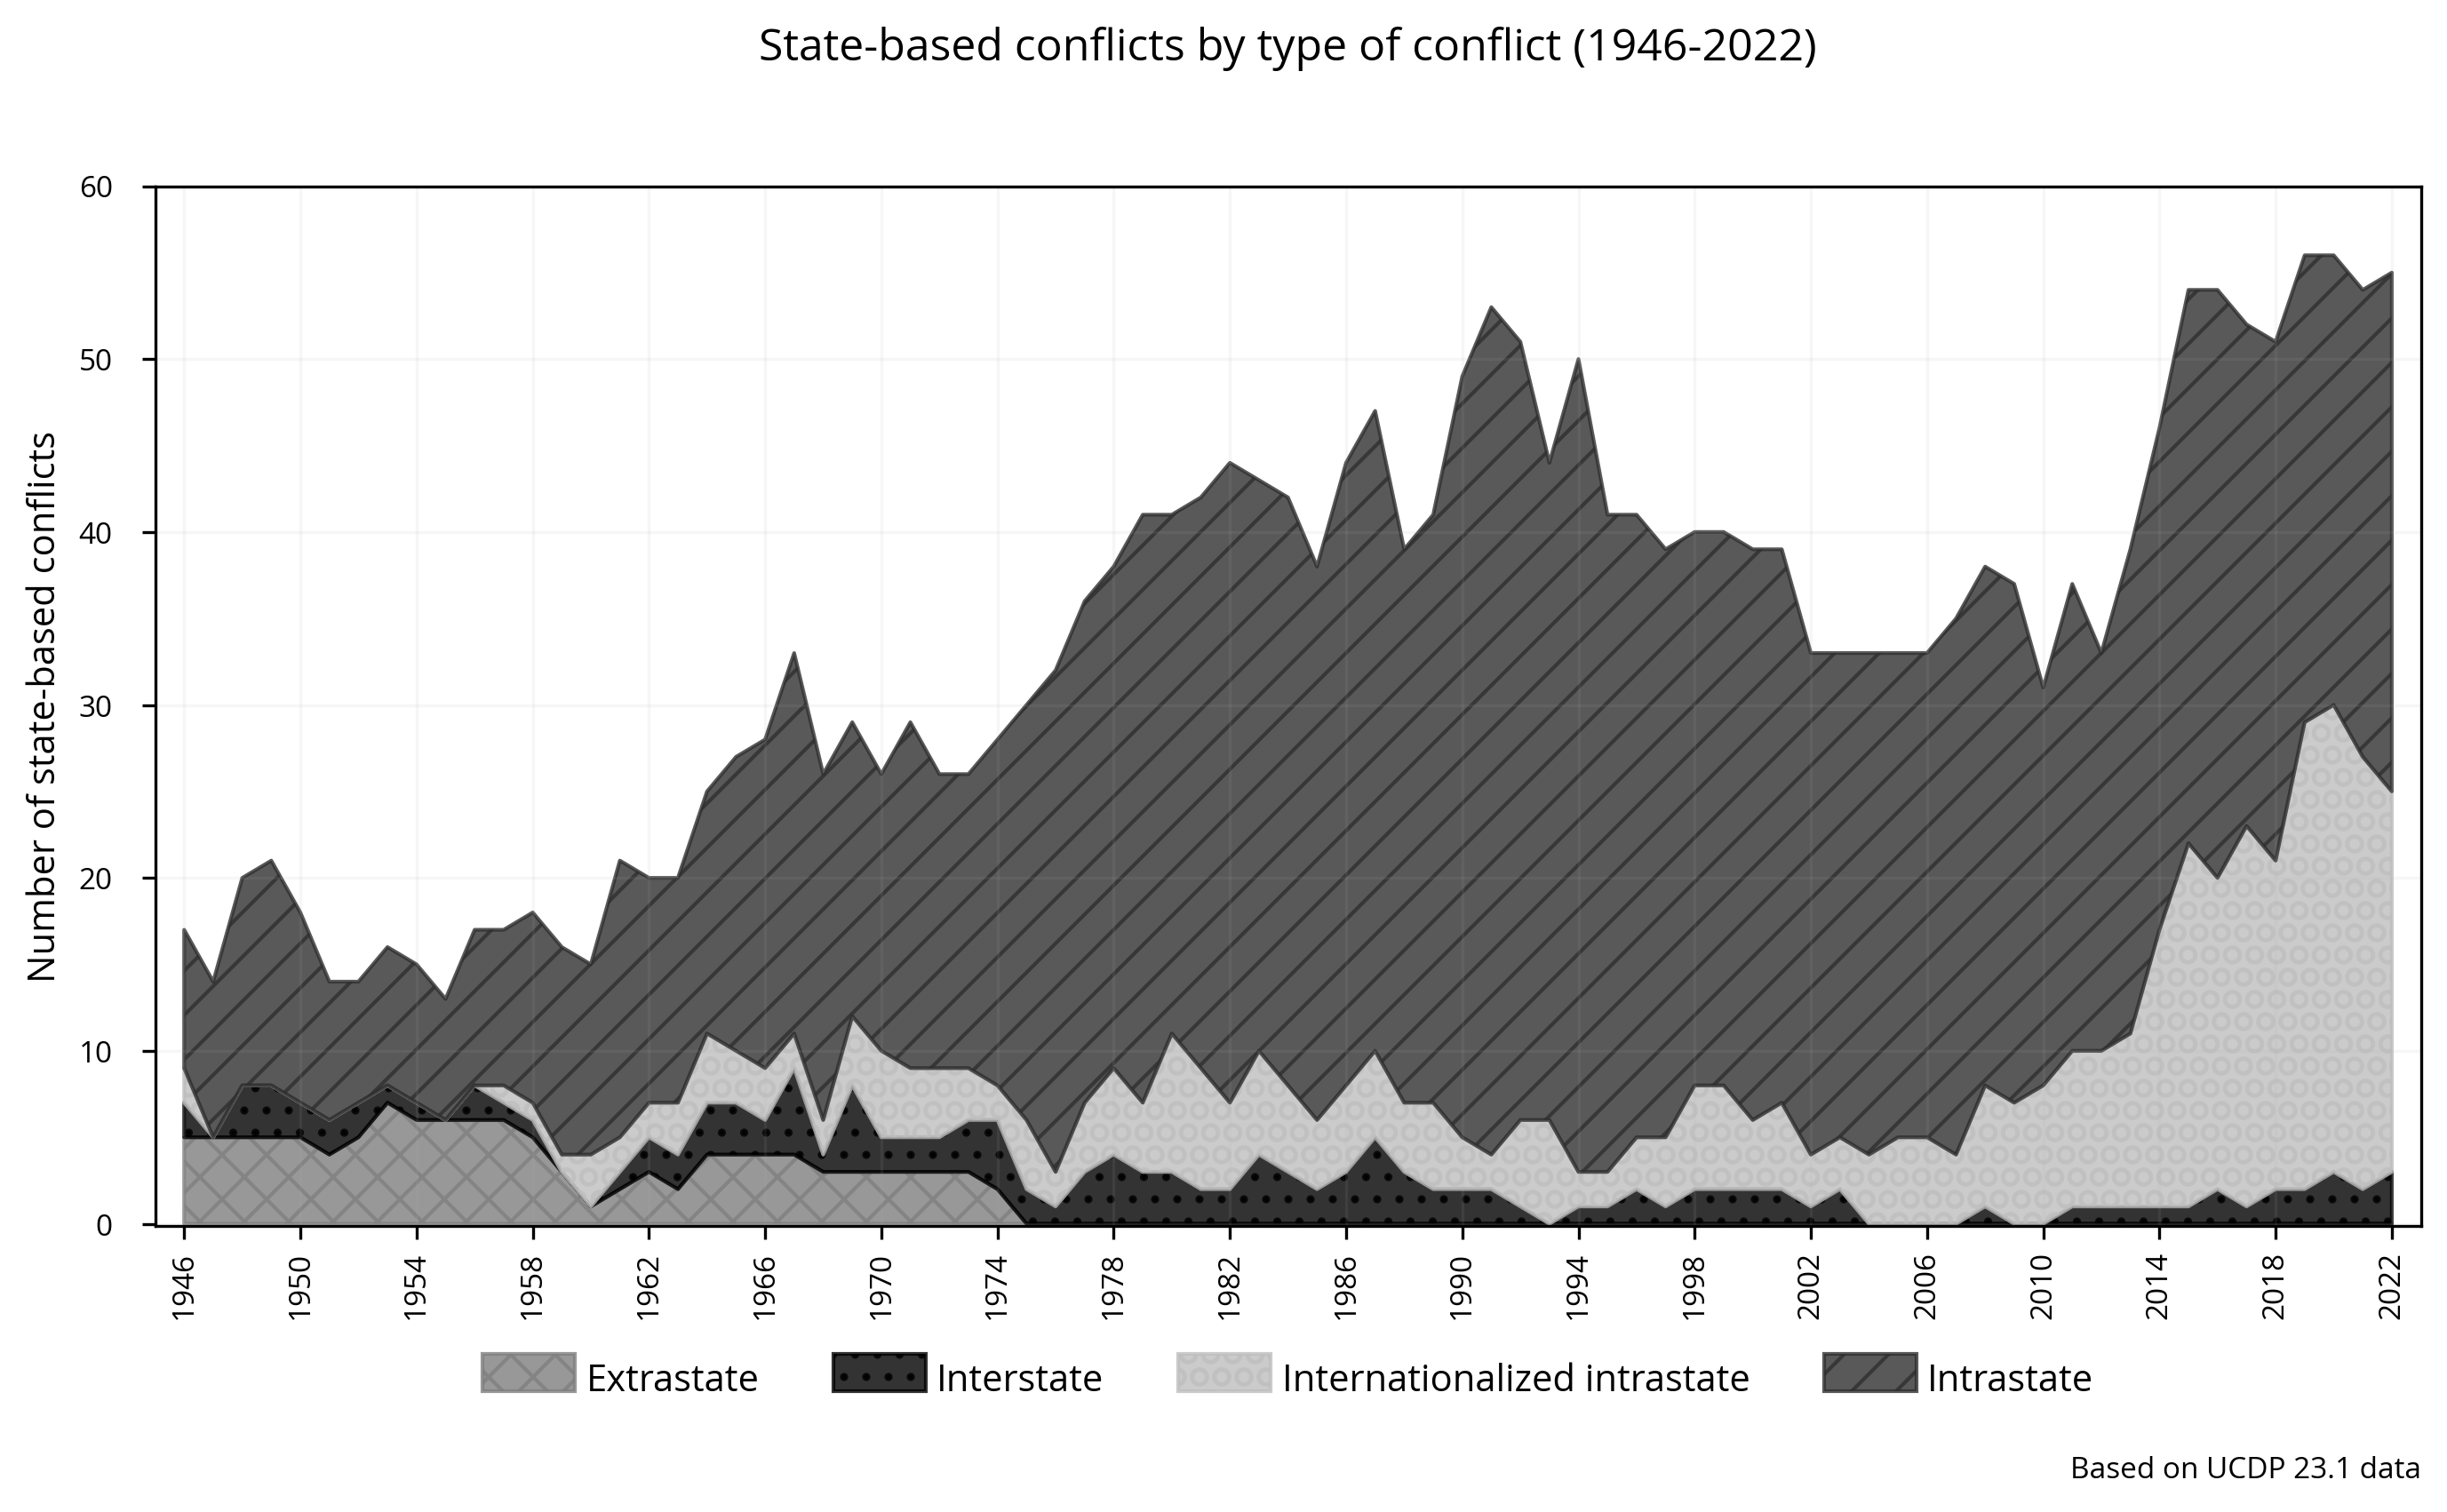
\includegraphics[width=\textwidth,height=\textheight,keepaspectratio]{armedconf_by_type.png}
	\end{figure}
\end{frame}

\begin{frame} 
	\frametitle{\LARGE{Conflict Locations}}
	\begin{figure}[ht!]
		\centering
		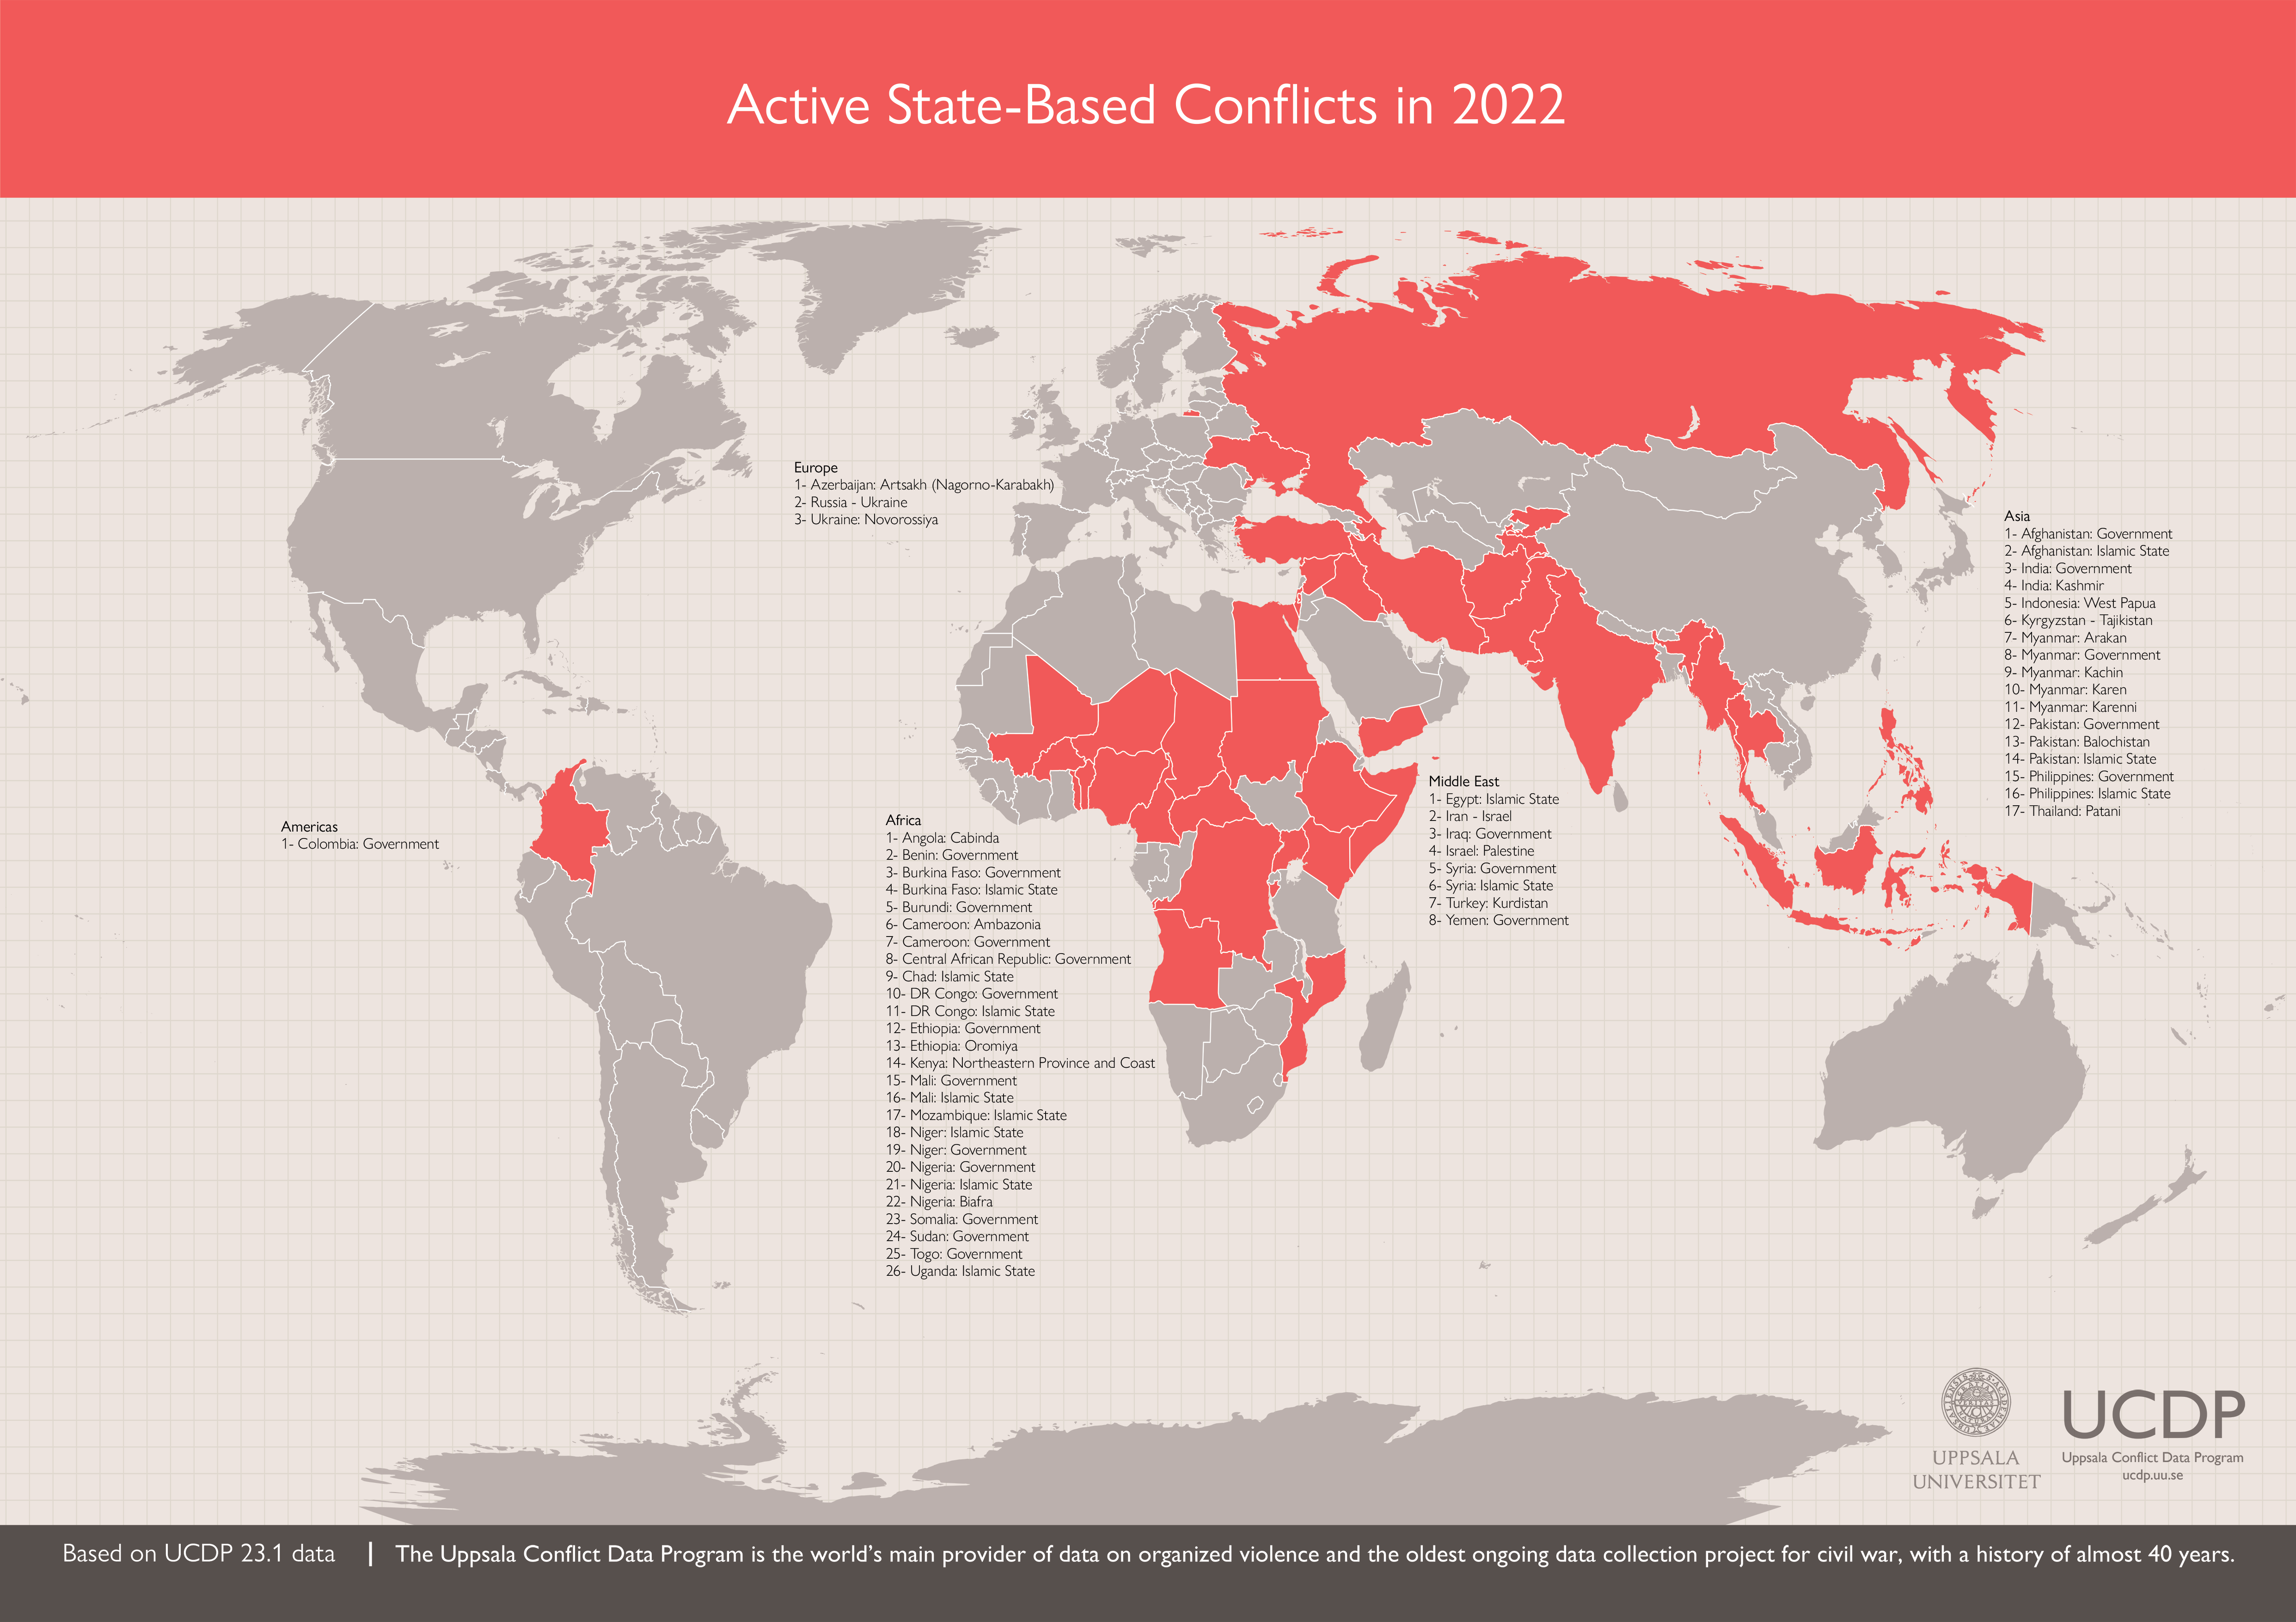
\includegraphics[width=\textwidth,height=\textheight,keepaspectratio]{WorldWap2022SB.png}
	\end{figure}
\end{frame}

\begin{frame} 
	\frametitle{\LARGE{Civil War Deaths 2}}
	\begin{figure}[ht!]
		\centering
		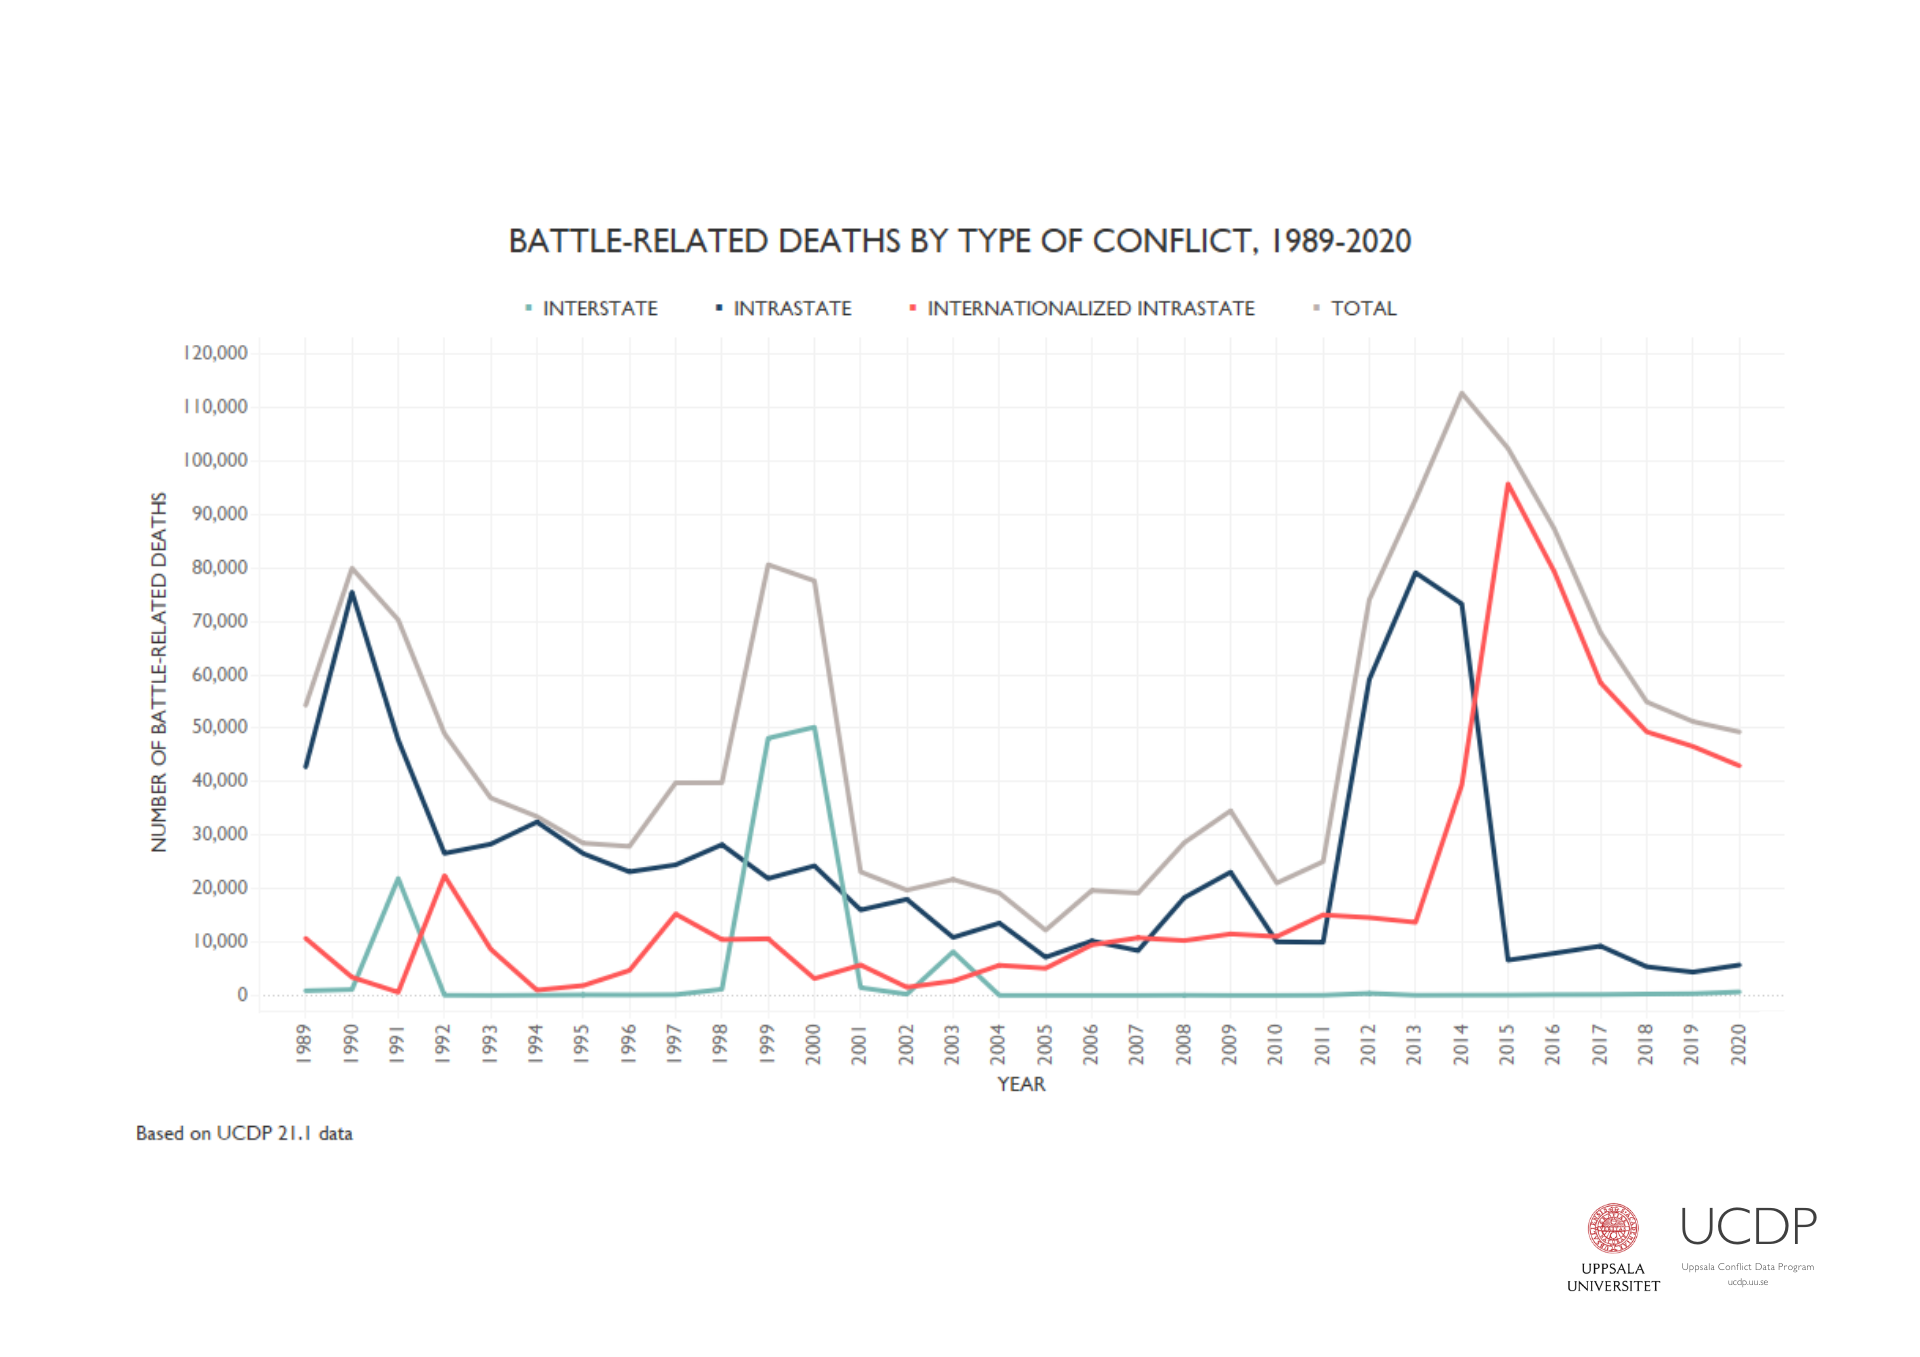
\includegraphics[width=\textwidth,height=\textheight,keepaspectratio]{brd_by_toc.png}
	\end{figure}
\end{frame}

\begin{frame} 
	\frametitle{\LARGE{Conflict Deaths}}
	\begin{figure}[ht!]
		\centering
		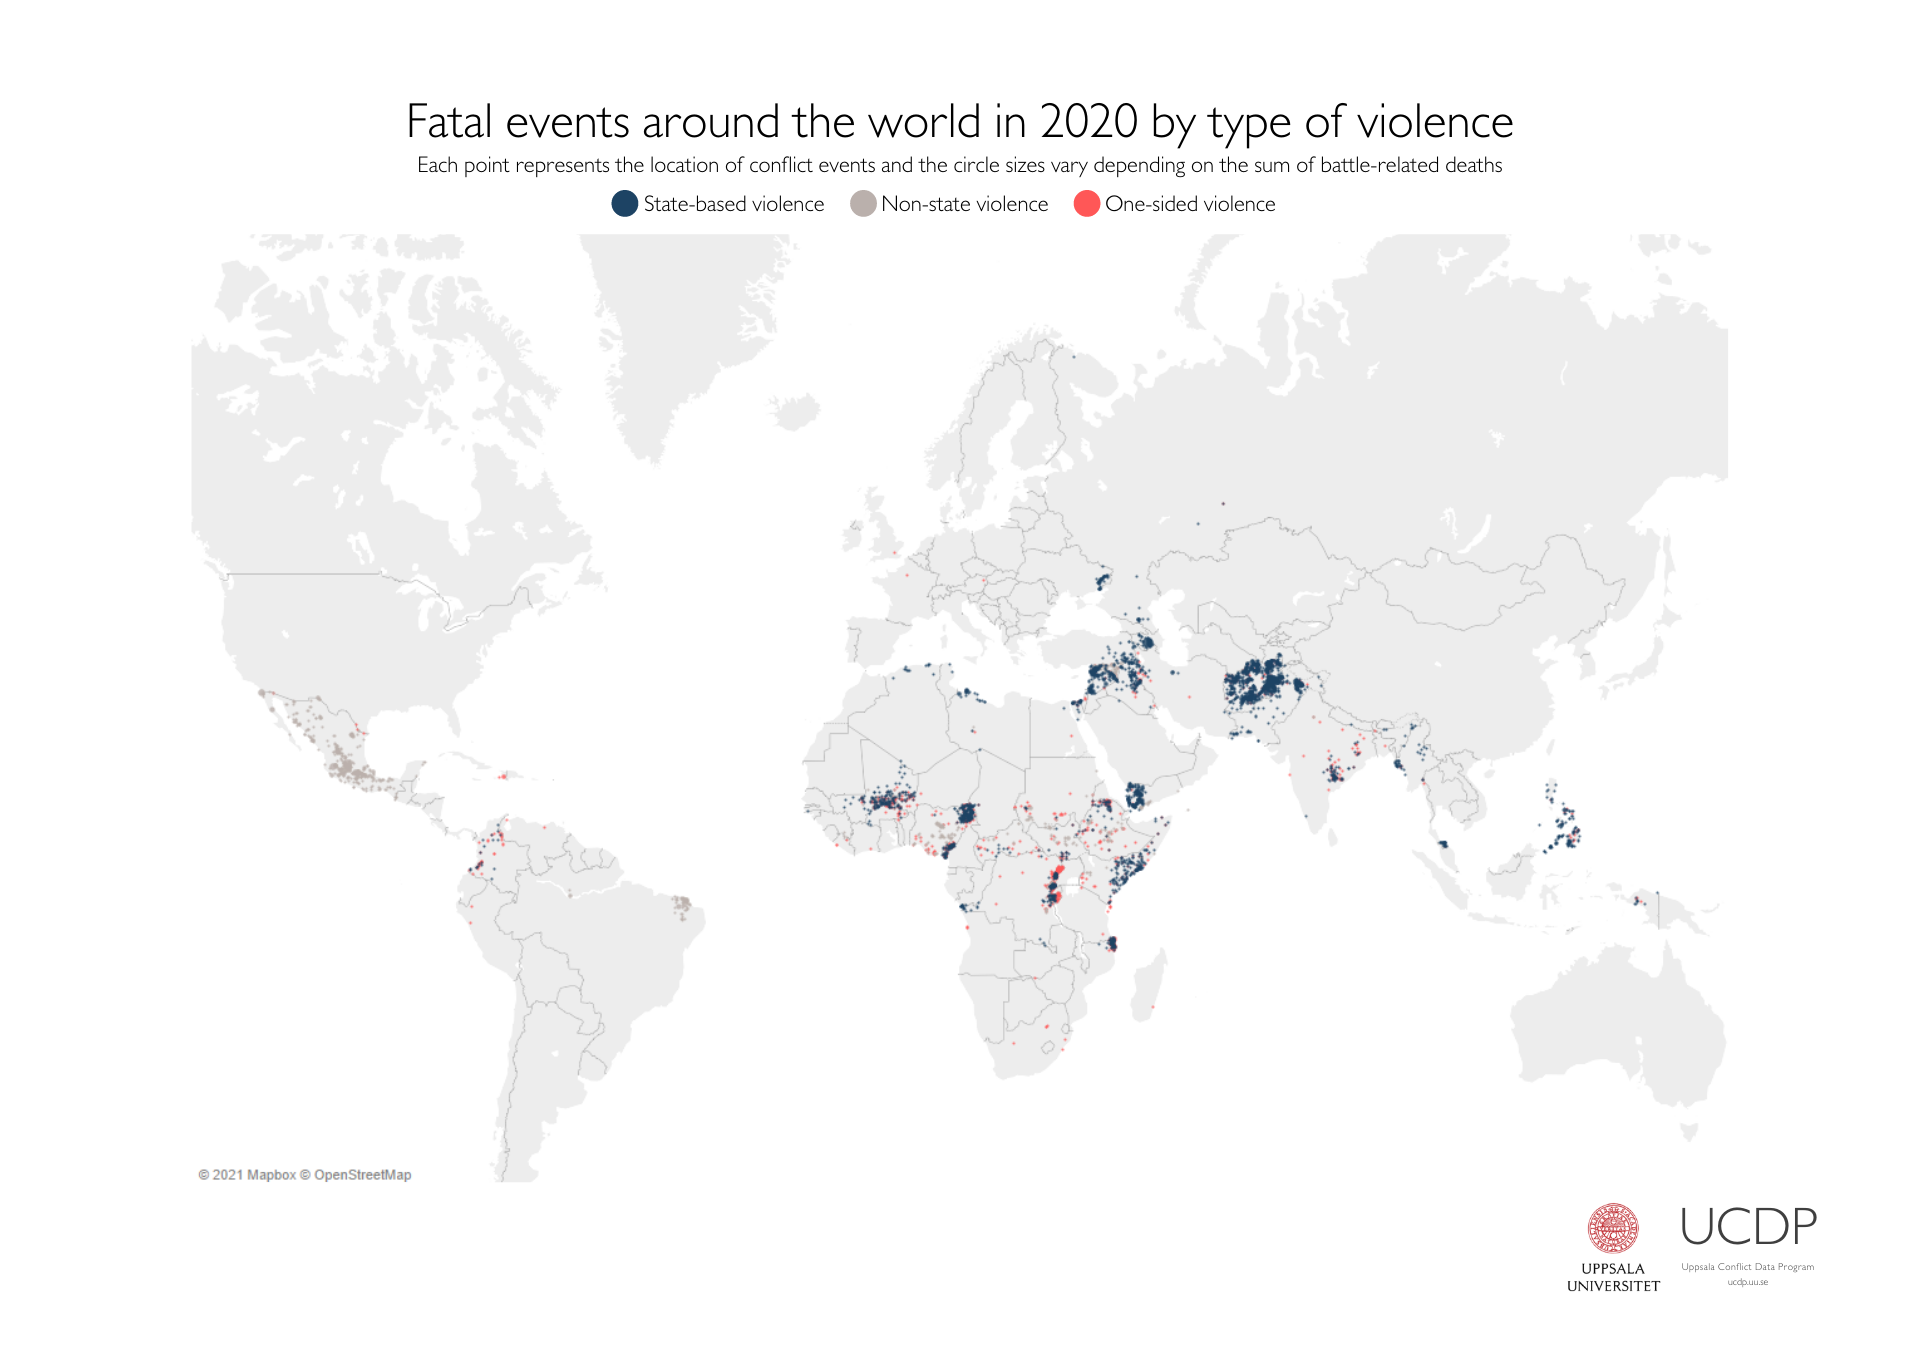
\includegraphics[width=\textwidth,height=\textheight,keepaspectratio]{worldin2020.png}
	\end{figure}
\end{frame}

\begin{frame} 
	\frametitle{\LARGE{US Civil War: Not Typical!}}
	\begin{figure}[ht!]
		\centering
		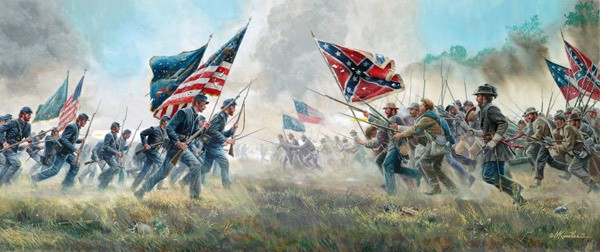
\includegraphics[width=\textwidth,height=\textheight,keepaspectratio]{uscivwar.jpeg}
	\end{figure}
\end{frame}

\begin{frame} 
\frametitle{\LARGE{Civil War: Why Fight?}}
As in interstate war, the occurrence of civil war is a puzzle. \pause
\begin{itemize}
		\item War is always costly, but in a civil war those costs are guaranteed to occur on the domestic front. \pause
		\item The state will generally be more powerful than any given rebel group, making chances of victory low. \pause
		\item Rebel groups must also overcome collective action problems.
\end{itemize}
\end{frame}

\begin{frame} 
\frametitle{\LARGE{Civil War Explanations}}
Political scientists have developed 3 general explanations for civil war at the group level, each of which supplements the others.
\begin{enumerate}
		\item Grievances
		\item Greed
		\item Rational choice frameworks
\end{enumerate}
\end{frame}

\begin{frame} 
	\frametitle{\LARGE{Civil War Explanation: Grievances}}
	\begin{itemize}
		\item Any state will contain citizens who are dissatisfied with government policy. \pause
		\item What separates the grievances explanation from that is that \textbf{these grievances are systemic, creating a domestic political situation with widespread inequality between groups}. \pause
		\item The state may economically marginalize certain groups, and this systematic exclusion from opportunities to gain wealth may provide an impetus to join rebel groups (especially if those groups pay). \pause
		\item These groups frequently form across ethnic and/or religious lines.
	\end{itemize}
\end{frame}

\begin{frame} 
	\frametitle{\LARGE{Civil War Explanation: Grievances}}
Any successful rebellion by such a marginalized group will presumably benefit the group as a whole, so how do they solve the collective action problem?
	\begin{itemize}
		\item Group norms of solidarity and cooperation may decrease free-riding. \pause
		\item Aspiring rebel leaders may use ethnic or religious ties to mobilize networks, and the closeness of those networks enables monitoring for free-riders. \pause
		\item Religious beliefs may both unify a group and provide non-material incentives to contribute.
	\end{itemize}
\end{frame}

\begin{frame} 
	\frametitle{\LARGE{Civil War Explanation: Grievances}}
However, civil war scholars have tended to argue that grievances are not the whole story. Why?
	\begin{itemize}
		\item \textbf{Every society has grievances of some kind, some of which rise to the level of systemic inequality, but not every society experiences civil war.} \pause
		\item While grievances may increase the probability of civil war, they are not enough to cause one by themselves. \pause
		\item Some work has also suggested that measures of grievance motivations really just measure susceptibility to mobilization.
	\end{itemize}
\end{frame}

\begin{frame} 
\frametitle{\LARGE{Civil War Explanation: Greed}}
	\begin{itemize}
		\item ``Greed" here is something of a misnomer. \pause
		\item This category is best described as a catch-all category for several factors: \pause
		\begin{enumerate}
			\item Opportunity costs of fighting
			\item Impact of resources on group formation and conflict incentives
			\item State-level elements that influence conflict (covered later in this presentation)
		\end{enumerate} 
	\end{itemize}
\end{frame}

\begin{frame} 
\frametitle{\LARGE{Greed: Opportunity Costs}}
\begin{itemize}
	\item \textbf{Opportunity cost}: in economics, the foregone gains from your next best option. \pause
	\begin{itemize}
		\item Ex: If job 1 pays you \$20,000/year and job 2 pays \$10,000 a year, job 1's opportunity cost is \$0, while job 2's opportunity cost is \$10,000. \pause
	\end{itemize}
	\item \textbf{At its core, this explanation argues that low opportunity costs for taking the ``job" of being a rebel make rebellion more likely.} \pause
	\item This implies that lower-income states should be more susceptible to civil wars.
\end{itemize}
\end{frame}

\begin{frame} 
	\frametitle{\LARGE{Greed: Violence and Collective Action}}
	Can violence in civil wars change the cost calculus of war?
	\begin{itemize}
		\item Thus far we've assumed war is costly for those who choose to fight in it. \textbf{But what if non-participation is costly too?} \pause
		\item Insurgency tends to be characterized by violence against non-combatants from both government and rebels. 
		\item If non-combatants are victimized, while combatants on either side get at least some protection from their chosen faction, then this changes the costs.
		\item \textbf{Participation in the conflict may be less costly than attempting to stay neutral, providing another solution to the collective action problem.}
	\end{itemize}
\end{frame}

%this is basically just Weinstein 2007
\begin{frame} 
	\frametitle{\LARGE{Greed: Resources}}
	\begin{itemize}
		\item Running a rebellion is expensive. \pause
		\item Some research (Weinstein 2007) has focused on whether lootable, fungible resources are available to rebel groups at their formation. This research argues that these resources shape the characteristics of the rebel group as well as its strategies of violence. \pause
		\item How? 
		\item Essentially, rebellions can be characterized into two types: those with an endowment of resources available at the beginning, and those without. 
	\end{itemize}
\end{frame}

\begin{frame} 
	\frametitle{\LARGE{Greed: Resources}}
First, consider the case of rebels with an initial endowment of resources.
	\begin{itemize}
		\item The presence of these economic incentives means that rebel recruiters can recruit based off of selective incentives. \pause
		\item ``Join us and we'll pay you / let you loot diamonds / etc."
		\item This leads to a rebellion composed primary of rebels who are self-interested, including those who joined purely for personal gain.
	\end{itemize}
\end{frame}

\begin{frame} 
	\frametitle{\LARGE{Greed: Resources}}
Now, consider the case of rebels without that initial endowment of resources.
	\begin{itemize}
		\item The lack of economic incentives means recruiters must find other ways to motivate participation. \pause
		\item Instead of the promise of payment, they will appeal to preexisting social capital to motivate fighters. \pause
		\item This frequently involves appeals to ethnic or religious in-groups (and this should remind you of the grievance mechanisms above). \pause
		\item Note that this should exclude purely opportunistic recruits. 
	\end{itemize}
\end{frame}

\begin{frame} 
	\frametitle{\LARGE{Greed: Resources}}
What does this mean for the rebel group's trajectory? Groups that formed via resource endowments will tend to:
		\begin{enumerate}
			\item Struggle to adequately control and discipline troops. \pause
			\item Respond to civilian resistance with authoritarian governance of their territories. \pause
			\item Likely struggle to limit indiscriminate violence by their soldiers.
		\end{enumerate}
\end{frame}

\begin{frame} 
	\frametitle{\LARGE{Greed: Resources}}
	What does this mean for the rebel group's trajectory? Groups that formed via social endowments will tend to:
	\begin{enumerate}
		\item More effectively shape and reinforce an organizational culture, leading to more  controlled troops. \pause
		\item Strike bargains with civilians in their territories, avoiding widespread civilian resistance. \pause
		\item Likely have less indiscriminate violence committed by their soldiers.
	\end{enumerate}
\end{frame}

\begin{frame} 
	\frametitle{\LARGE{Civil War Explanations: Rational Choice}}
	This group of explanations applies Fearon's (1995) bargaining model to civil wars. \pause
	\begin{itemize}
		\item \textbf{Incomplete information and incentives to misrepresent}: this argues that the usual incentives to misrepresent are just as present, if not even worse.
		\begin{itemize}
			\item Very difficult for state to gauge rebel capabilities. \pause
			\item Rebel groups generally unable to demonstrate capacity without revealing their locations to the state. \pause
			\item Less pre-war diplomacy is possible, meaning that less information is shared. \pause
			\item Sovereignty concerns shrink (eliminate?) the bargaining range.
		\end{itemize}
	\end{itemize}
\end{frame}

\begin{frame} 
	\frametitle{\LARGE{Civil War Explanations: Rational Choice}}
	\begin{itemize}
	\item \textbf{Incomplete information and incentives to misrepresent}: a weak explanation for a few key reasons.
	\begin{itemize}
		\item Average civil war lasts 6-7 years. Lots of time to communicate information. \pause
		\item Rebel groups always substantially weaker than state governments.
	\end{itemize}
	\end{itemize}
\end{frame}

\begin{frame} 
	\frametitle{\LARGE{Commitment Problems in Civil War}}
\textbf{Commitment problems} can also occur:
	\begin{itemize}
			\item Shifting power: downturns in economy create incentives for rebels to fight as they gain recruits while the state weakens. \pause
			\item \textbf{States cannot credibly commit to honor the terms of an agreement once the rebels disarm.} \pause 
			\item Rebel leaders cannot fully control their members, so cannot credibly commit to the cessation of violence. \pause
			\item These commitment problems make peace agreements that end civil wars difficult, and often require third-party enforcement.
	\end{itemize}
\end{frame}

\begin{frame} 
	\frametitle{\LARGE{Civil War Explanations: Rational Choice}}
	\begin{itemize}
		\item \textbf{Commitment problems}: considered a much stronger explanation than information problems, especially because of two of those factors:
		\begin{itemize}
			\item Rebels will not trust the state not to retaliate against them after disarmament, which any peace deal will generally require. \pause
			\item One or both sides may anticipate changes to the balance of power (especially in favor of the state) that render a deal non-credible.
		\end{itemize}
	\end{itemize}
\end{frame}


\begin{frame} 
	\frametitle{\LARGE{Civil War Explanations: Rational Choice}}
 \textbf{Indivisibility}: also a strong explanation.
		\begin{itemize}
			\item States may conceptualize sovereignty as an indivisible good, preventing them from making any meaningful concessions to rebel groups. \pause
			\item States may be especially likely to do this if they contain many other groups of potential rebels. \pause
			\item If a state makes concessions to placate one group, others may conclude that violent conflict is an effective way to influence the state.
		\end{itemize}
\end{frame}

\begin{frame} 
	\frametitle{\LARGE{Summary (So Far)}}
	\begin{itemize}
		\item \textbf{Grievance explanations}: explains group motivations in particular cases, but not sufficient to explain why civil war occurs in some cases but not others. \pause
		\item \textbf{``Greed" explanations}: can explain group behavior and characteristics, as well as differences in how they treat civilians. \pause
		\item \textbf{Rational choice explanations}: commitment problems provide strong incentives to keep fighting, as does indivisiblity.
	\end{itemize}
\end{frame}

\begin{frame} 
	\frametitle{\LARGE{Additional Causes}}
	\begin{itemize}
		\item Greed vs. grievance was a long-running debate in IR. \pause
		\item Eventually, scholars recognized the impact of both on civil wars. \pause
		\item This narrow framework can also obscure some causes that don't fit neatly into either category, which is why the textbook groups causes by level:
		\begin{itemize}
			\item Group-level
			\item State-level
			\item International-level
		\end{itemize} 
	\end{itemize}
\end{frame}

\begin{frame} 
\frametitle{\LARGE{Group-Level Factors}}
\begin{itemize}
		\item This is primarily concerned how groups overcome their greatest initial obstacle: the collective action problem. \pause
		\item Strong in-group ties that facilitate collective action via norms of participation, monitoring for free-riders, and social capital all come into play here. \pause
		\begin{itemize}
		\item Ideology, ethnicity, tribal motivations, religious motivations. \pause 
		\end{itemize}
		\item In the absence of those factors, groups can use material incentives or forced recruitment. \pause
		\item Most grievance, greed, and rational choice causes apply at the group level.		
\end{itemize}
\end{frame}

\begin{frame} 
\frametitle{\LARGE{Country-Level Factors}}
 Which type of regime is most likely to experience civil war?\pause
\begin{itemize}
		\item Autocracy: individuals are more likely to be aggrieved and excluded from the political process, while the state is likely to have a repressive apparatus. \pause
		\\~\\
		\item Democracy: a democratic state may have less repressive capacity, but citizens can also express and address their grievances via the electoral process. \pause 
		\\~\\
		\item \textbf{Anocracy/mixed regime}: neither fully autocratic nor fully democratic, these regimes lack both the avenues for participation and repressive capacity.
\end{itemize}
\end{frame}

%https://www.pewresearch.org/fact-tank/2019/05/14/more-than-half-of-countries-are-democratic/ft_19-05-02_democracyupdate_map/
\begin{frame} 
	\frametitle{\LARGE{Anocracy Over Time}}
	\begin{figure}[ht!]
		\centering
		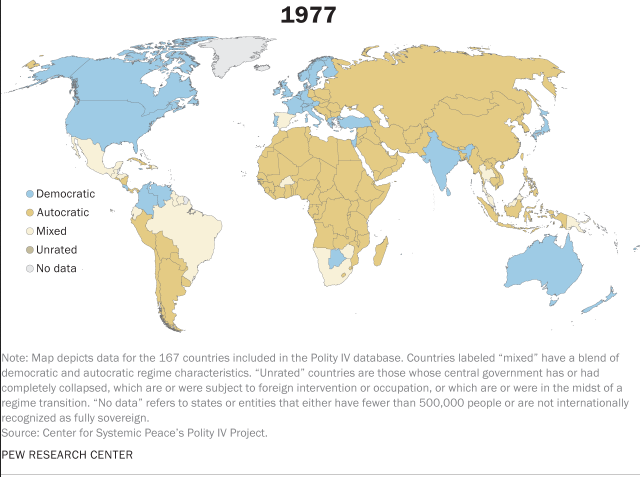
\includegraphics[width=\textwidth,height=.9\textheight,keepaspectratio]{anocracy1.png}
	\end{figure}
\end{frame}

\begin{frame} 
	\frametitle{\LARGE{Anocracy Over Time}}
	\begin{figure}[ht!]
		\centering
		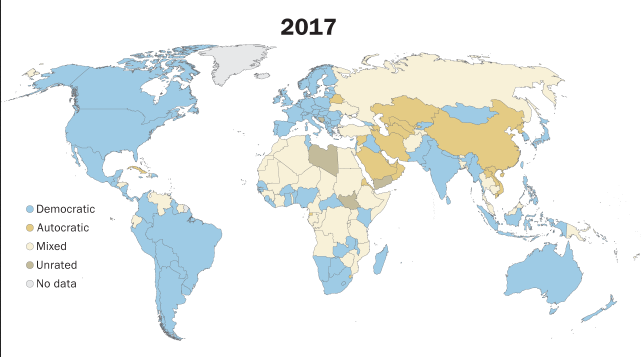
\includegraphics[width=\textwidth,height=\textheight,keepaspectratio]{anocracy2.png}
	\end{figure}
\end{frame}


\begin{frame} 
\frametitle{\LARGE{Other Country-Level Factors}}
\begin{itemize}
		\item \textbf{Wealth}: poverty makes individuals more desperate (lower opportunity costs of joining rebellion) and poor states are usually weaker than rich countries (meaning the state may struggle to suppress a rebellion). \pause
		\item \textbf{Population}: more populous countries have a larger recruitment pool; larger population also allows the rebels to hide in it. \pause
		\item \textbf{Size}: the larger the area, the harder to police (especially if lower state capacity). \pause 
		\item \textbf{Terrain}: mountainous or jungle terrain makes hiding from the state easier.
\end{itemize}
\end{frame}

\begin{frame} 
	\frametitle{\LARGE{International Factors}}
	\begin{itemize}
		\item While states violently oppose rebel groups in their own territory, this does not necessarily mean they oppose all rebel groups in other states. \pause
		\item States may support rebel groups within a rival's territory to weaken their rival. \pause
		\item States may also support rebels with whom they share ethnic or ideological ties. \pause
		\item Support can range from diplomatic support up to sending weapons and troops. 
	\end{itemize}
\end{frame}

\begin{frame} 
\frametitle{\LARGE{International Factors}}
\begin{itemize}
		\item Any external support for at least one side makes a civil war \textbf{internationalized}: foreign government(s) supporting at least one side with supplies or troops. \pause
		\item Some internationalized civil wars are \textbf{proxy wars}: at least 2 outside states each back opposing sides of a civil war. \pause
		\item Diaspora groups can also lend economic support to groups (i.e. Irish Americans supporting the IRA).\pause
		\item \textbf{Note that most civil wars do not turn into internationalized proxy wars}, but those wars attract disproportionate media coverage...
\end{itemize}
\end{frame}

\begin{frame} 
	\frametitle{\LARGE{Internationalized Example: Syria}}
	\begin{itemize}
		\item 2011: protests against the Assad regime turn violent; rebel groups coalesce. \pause
		\item As conflict continues, US provides limited support to rebels and strikes deal with Russia to dismantle Syrian chemical weapons.\pause
		\item Rebel groups fragment and begin to fight each other, marking the formation of ISIS.\pause
		\item Turkey, US, Saudi Arabia start to intervene on the side of the rebels.\pause
		\item Iran and Russia provide military support to the Syrian government.
	\end{itemize}
\end{frame}

\begin{frame} 
	\frametitle{\LARGE{Internationalized Example: Syria}}
	\begin{itemize}
		\item Conflict continues as US supports (then later abandons) Kurdish rebels while Turkey starts attacking said rebels, later moving its own forces across the northern border, while still opposing the Syrian government. \pause
		\item Some spillover into Lebanon, while Israel has also struck Iranian forces and Hezbollah near its borders. \pause
		\item Russian intervention continues, pulling the Syrian government back from the brink of collapse. \pause
		\item Fighting between regime and rebels winds down as regime retakes most of its territory. \pause
		\item At present, violence has decreased from previous levels but skirmishes continue, involving Turkish military forces and assorted factions within Syria.
		
	\end{itemize}
\end{frame}

\begin{frame} 
	\frametitle{\LARGE{Internationalized Example: Syria}}
	\begin{figure}[ht!]
		\centering
		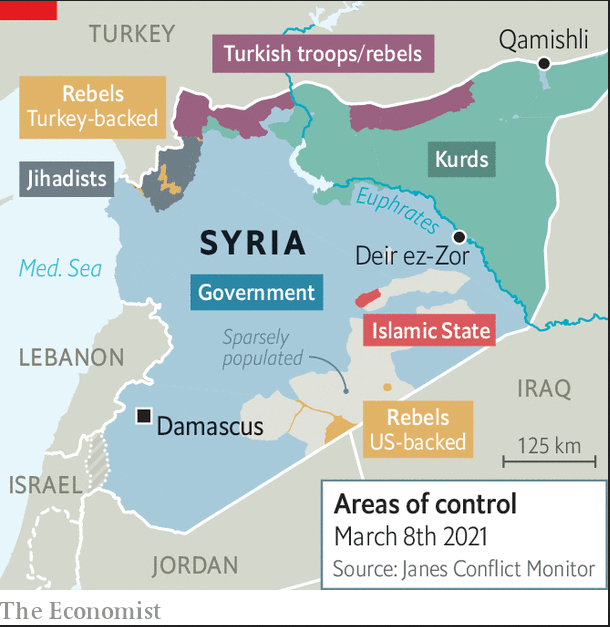
\includegraphics[width=\textwidth,height=0.9\textheight,keepaspectratio]{Syria2021.png}
	\end{figure}
\end{frame}

%
\begin{frame} 
	\frametitle{\LARGE{\href{https://acleddata.com/2022/12/01/the-state-of-syria-q2-2022-q3-2022/}{ACLED Map} of Syria}}
	\begin{figure}[ht!]
		\centering
		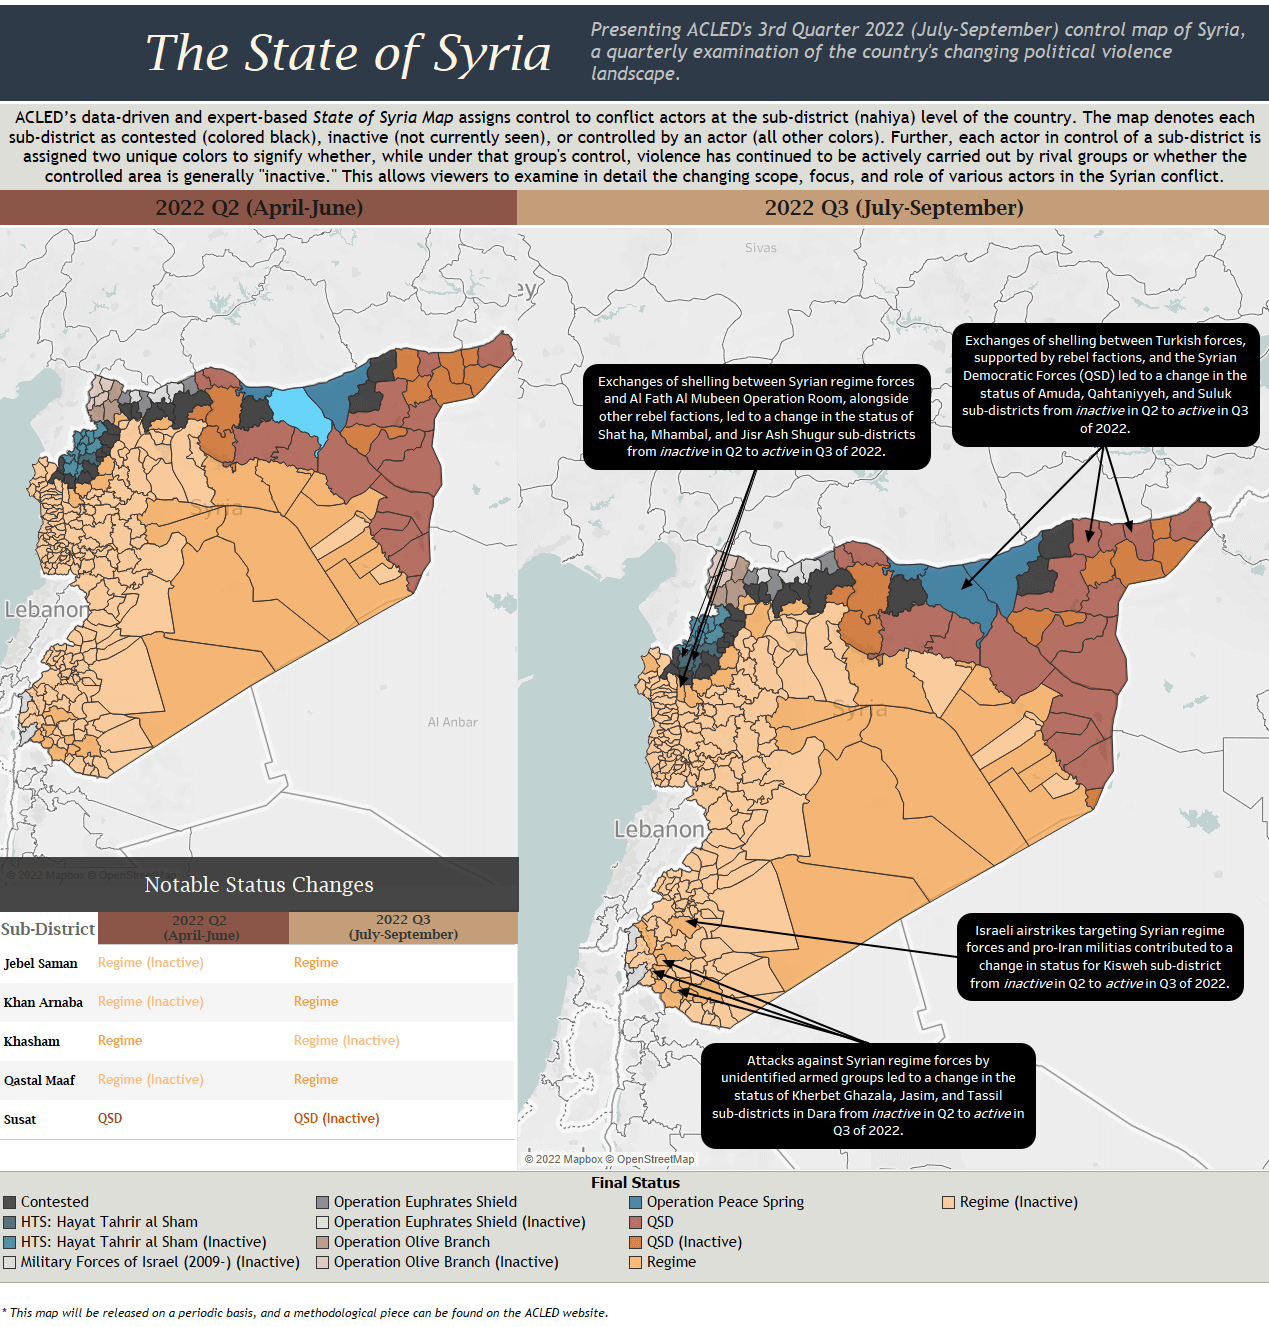
\includegraphics[width=\textwidth,height=\textheight,keepaspectratio]{Syria-Q3-2022.png}
	\end{figure}
\end{frame}



\begin{frame} 
	\frametitle{\LARGE{Summary}}
	\begin{itemize}
		\item Civil wars occur within a state, as the government fights rebel group(s). \pause
		\item Rebels typically motivated to fight by a combination of grievances, material incentives, and social ties. \pause
		\item A rational-choice perspective shows that civil wars are exacerbated by commitment and indivisibility problems, while violence against non-combatants may change the costs of war. \pause
		\item State-level factors such as state capacity and terrain can also impact rebellion viability. \pause
		\item Civil wars can draw the attention of other international actors.
	\end{itemize}
\end{frame}

\begin{frame} 
	\frametitle{\LARGE{Closing Question}}
	\centering
	\Large{What about civilians?} 
\end{frame}



\end{document}
